\subsection{Wyzwania i metody zapewniania bezpieczeństwa systemów autonomicznych i sieci IoT}

\subsubsection{Definicja IoT}

Jednym z kluczowych zjawisk przyczyniającym się do procesu nagłego przyrostu ilości i źródeł danych jest Internet przedmiotów (ang. \textit{Internet of Things}). Według tej koncepcji, \textbf{różnego typu urządzenia osadzone w urządzeniach codziennego użytku}(np. odkurzacze, żarówki, instalacje grzewcze), czy też w maszynach przemysłowych, zbierają dane o otoczeniu, czy samym procesie w którym uczestniczą, a ponadto \textbf{mają możliwość komunikacji pomiędzy sobą, ale również z jednostką centralną}, jeśli taka występuje. Wprowadza to nowy wymiar w możliwościach automatyzacji procesów i kreuję nową przestrzeń do tworzenia się złożonych, inteligentnych systemów.

\begin{figure}[H]
	\centering
	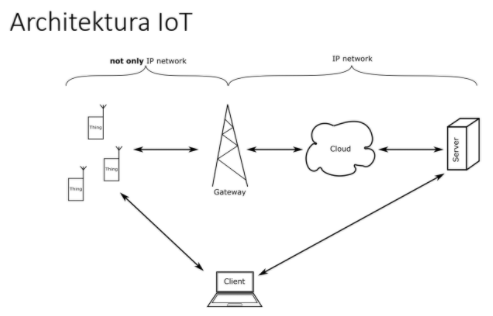
\includegraphics[width=0.7\linewidth]{S8.png}
	\caption{Architektura IoT}
\end{figure}

\subsubsection{Wyzwania IoT}

\begin{itemize}
	\item Trudne \textbf{zapewnienie fizycznej ochrony} sprzetu,
	\item \textbf{Bezpieczeństwo danych wysłanych} przez urządzenia i przechowywanych w chmurze
	\item \textbf{Domyślne hasła urządzeń},
	\item \textbf{Domyślny brak filtrowania ruchu},
	\item \textbf{Brak zasobów do implementacji} silnych \textbf{zabezpieczeń},
	\item Zapewnienie \textbf{bezpiecznego połączenia} urządzenia \textbf{z chmurą obliczeniową}
\end{itemize}

\subsubsection{Mechanizmy bezpieczeństwa sieci IoT}

\begin{itemize}
	\item \textbf{Identyfikacja} (np. Po IMEI urządzenia) i autentykacja wszystkich urządzeń w sieci w celu ochrony przed podszywaniem się pod urządzenia,
	\item \textbf{Kontrola dostępu pomiędzy urządzeniami}:
	\begin{itemize}
		\item wykorzystywanie \textbf{VPN}, tunelowania L2TP (protokół tunelowania warstwy drugiej) lub IPsec,
		\item Konfiguracja dostępu do zasobów w oparciu o kontekst działania – limitowanie dostępu tylko do potrzebnych informacji
	\end{itemize}
	\item \textbf{Szyfrowanie} przesyłanych danych
	\item \textbf{Utrzymanie dostępności} zasobów:
	\begin{itemize}
		\item Implementacja przetestowanych, certyfikowanych i  ustandaryzowanych technologi komunikacji, np. GSM, UMTS, LTE, 
		\item Technologie radiowe IoT:
		\item konfiguracja odpornych na przeciążenia i ataki topografii sieci, 
		\item monitorowanie na żywo 24/7 zasobów sieci i wydajności urządzeń
		\item \textbf{Niezawodność transmisji}
		\begin{itemize}
			\item \textbf{nadmiarowość}
			\item \textbf{wykrywanie błędów}
			\begin{itemize}
				\item ACK
				\item żądania retransmisji
			\end{itemize}
			\item \textbf{korygowanie błędów}
		\end{itemize}
	\end{itemize}
	\item \textbf{Testy bezpieczeństwa} kodu źródłowego urządzeń IoT (wycieki pamięci, przepełnienie bufora)
	\item Zapewnienie \textbf{aktualizacji} bezpieczeństwa wykorzystywanego oprogramowania
	\item Unikanie \textbf{inicjacji połączenia przez urządzenia} – jedynie przez firewalle, proxy lub listy dostępu w celu ograniczenia ryzyka ataku na systemu wewnętrzne
	\item \textbf{Oddzielenie sieci urządzeń od sieci serwerów} współdzieloną, zabezpieczoną firewallem siecią przekazywania danych
\end{itemize}

\subsubsection{System autonomiczny}

\begin{figure}[H]
	\centering
	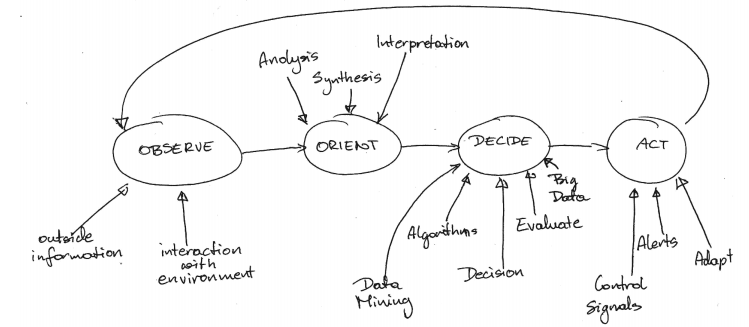
\includegraphics[width=0.7\linewidth]{S8_2.png}
	\caption{Schemat systemu autonomicznego}
\end{figure}

\subsubsection{System autonomiczny - wyzwania}

\begin{itemize}
	\item prawa jednostki vs. prawa ogółu
	\begin{itemize}
		\item Social Credit System w Chinach
	\end{itemize}
	\item \textbf{prawa robotów} (sztucznej inteligencji)
	\item \textbf{prawo karne}
	\begin{itemize}
		\item egzekwowanie
		\item zapobieganie
	\end{itemize}
	\item \textbf{prawo pracy}
	\item \textbf{prawo własności intelektualnej}
	\item \textbf{etyka}
\end{itemize}

\subsubsection{Wyzwania technologiczne}

\begin{itemize}
	\item \textbf{gromadzenie danych}
	\begin{itemize}
		\item sensory
		\item sieci komunikacyjne
		\item przechowywanie
	\end{itemize}
	\item \textbf{przetwarzanie danych}
	\begin{itemize}
		\item dostępność
		\item algorytmy
	\end{itemize}
	\item \textbf{autonomiczność pracy}
	\begin{itemize}
		\item zasilanie
		\item niezawodność
	\end{itemize}
\end{itemize}

\begin{figure}[H]
	\centering
	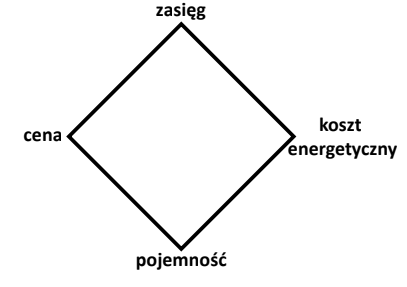
\includegraphics[width=0.4\linewidth]{S8_1.png}
	\caption{Kompromis}
\end{figure}

